\documentclass[a4paper]{jpconf}
\usepackage{graphicx}
\usepackage{amsmath}
\usepackage{amssymb}
\usepackage{array}
\begin{document}

\title{Lossless Transmission for Geo-Distributed AI Computing via LSQ-Sketch and APN-Aware SRv6 Backpressure}


\author{Sheng Haiyan$^1$, Yang Yong$^2$, Liu Ye$^1$,Yan Jiayao$^1$, Fei Shuoyao$^1$}


\address{$^1$ Century College, Beijing University of Posts and Telecommunications, Beijing, 100876, China}
\address{$^2$ China Mobile Communications Group Beijing Co., Ltd., Beijing, 100032, China}
\ead{yangyongbupt168@foxmail.com}


\begin{abstract}
The expanding scale of Large Language Model (LLM) training necessitates a shift toward geo-distributed, disaggregated computational architectures. However, deploying Remote Direct Memory Access (RDMA) over conventional Wide Area Networks (WANs) introduces severe challenges, including latency-induced flow-control failures, load imbalances from elephant-flow polarization, and inadequate multi-tenant isolation. To address these bottlenecks, we propose a lossless transmission architecture tailored for geo-distributed AI computing that operates synergistically across three network planes. At the data plane, a hardware-traffic co-design employs a Load-Store Queue (LSQ) to resolve SRAM read-write dependencies at Terabit-per-second (Tbps) line rates. This structural enhancement enables out-of-order-free micro-flow scheduling via Unequal Cost Multi-Path (UCMP) routing, effectively accommodating the ON/OFF burst patterns of AI workloads. Within the control plane, a tenant-level elastic backpressure mechanism leveraging SRv6 End.X.PFC in-band signaling strictly confines fault domains and prevents global deadlocks. At the management plane, Application-aware Networking (AAN) coupled with slice sub-interfaces guarantees physical hard isolation and data-compliance fencing. Empirical evaluations on a 100-kilometer production WAN demonstrate that this architecture improves link utilization from 45\% to over 90\% while reducing 99th-percentile tail latency and maximum queue depth by approximately 68\%. Furthermore, it substantially decreases Job Completion Time (JCT) for prevalent LLM workloads, restricting computing efficiency degradation to under 1.8\%, thereby establishing a robust, deterministic network foundation for high-performance geo-distributed AI computing.
\end{abstract}

\noindent{\bf Keywords.} Geo-Distributed AI Computing, Lossless Transmission, Hardware-Algorithm Codesign, Application-aware Networking (AAN)

\section{Introduction}


Trillion-parameter LLMs demand massive compute, exposing single-datacenter (DC) constraints [1]. Consequently, geo-distributed AI across wide-area networks (WANs) has emerged as a critical shift [2]. Privacy regulations mandate disaggregated paradigms---local data, remote training---requiring high throughput, lossless transmission, and multi-tenant isolation.


Extending intra-DC RoCEv2 to WANs introduces severe challenges [3]. Increased round-trip times (RTT) and bandwidth-delay products (BDP) [4] degrade congestion control, exacerbating PFC deadlocks and Head-of-Line (HoL) blocking [5]. Additionally, AI elephant flows cause severe load imbalance under conventional Equal-Cost Multi-Path (ECMP) routing [6]. Meanwhile, WAN latency renders host-side scheduling impractical, and traditional IP networks lack application awareness to enforce SLAs.


To overcome these bottlenecks, we propose a cross-plane lossless WAN architecture. The data plane leverages a Load-Store Queue (LSQ) and UCMP routing for reordering-free, network-side micro-flow scheduling. The control plane utilizes SRv6 End.X.PFC signaling for tenant-level backpressure, preventing global deadlocks. Finally, the management plane integrates APN with network slicing for strict data fencing. Together, this establishes a deterministic, application-aware foundation for geo-distributed AI.


\section{Overall Architecture of the Lossless Transmission Mechanism and Multi-Dimensional Data-Network Synergy}


To address the extreme performance challenges imposed by AI computing services on wide-area networks (WANs) while satisfying the stringent security and isolation requirements of data circulation scenarios, this paper proposes a multi-dimensional intelligent WAN framework based on data--network synergy.


The proposed architecture consists of three tightly coupled layers, whose core design principle is the deep integration of computing-resource awareness with network-routing intelligence.


\begin{figure}[h]
\begin{center}
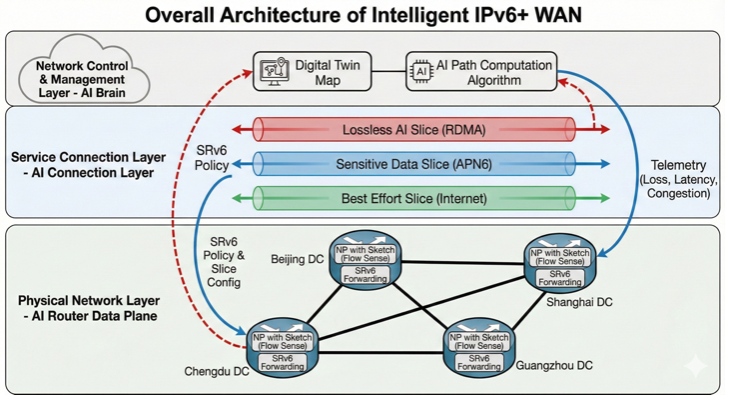
\includegraphics[width=30pc]{fig1.png}
\end{center}
\caption{\label{fig1}Overall Architecture of the Mechanism}
\end{figure}


The first layer is the Physical Network Layer (AI Router Data Plane), which establishes a highly flexible networking infrastructure based on programmable SRv6. This layer introduces next-generation AI routers equipped with endogenous intelligence capabilities, enabling high-speed traffic feature extraction and hardware-level Sketch-based statistical inference directly within the Network Processing Unit (NPU) [7].


The second layer is the Service Connection Layer (AI Connection Layer), which leverages the IPv6 Extension Header framework to embed APN identifiers (APN IDs) and Slice IDs carrying rich service semantics. This design enables the network to differentiate and manage traffic flows with heterogeneous Service Level Agreement (SLA) requirements at the protocol level.


The third layer is the Network Control Layer (AI Brain), which functions as the central intelligence of the WAN architecture. This layer deploys an intelligent Software-Defined Networking (SDN) controller with a global network view and a high-precision digital network map. By utilizing large-scale real-time telemetry data, the controller dynamically computes globally optimized congestion-free paths and distributes SRv6 policies with explicit routing information, thereby enabling intelligent orchestration and fine-grained scheduling of network traffic [8].


\section{Statistical Algorithm Innovation and Scheduling Theory Tailored for High-Speed NPU Hardware}


Under the severe environment of long-distance WAN transmission, resolving the congestion and hash collisions caused by elephant flows is key to improving overall network throughput. Rather than modifying macroscopic statistical algorithms, this paper proposes a hardware-based statistical algorithm and micro-flow scheduling theory tailored for ultra-high-speed network processing.


\subsection{Hardware-Traffic Co-design of LSQ and Micro-cache Based on the ON/OFF Traffic Model}


While Count-Min Sketch is a well-established matrix-based approach for network traffic filtering [9], high-speed network devices traditionally employ LSQs to mitigate Read-After-Write (RAW) hazards and micro-caches for preprocessing acceleration [10]. These architectural primitives have been extensively validated in high-performance designs like SPArch [11]. Building upon these existing components, our primary contribution is a novel hardware-traffic co-design framework specifically tailored to the wide-area burst characteristics of large AI models.


In distributed training, gradient synchronization mechanisms dominate network behavior. Assuming the model parameter size is $P$ and the total number of GPU computing nodes is $W$, during a single Ring All-Reduce iteration, the data volume each node needs to send and receive theoretically reaches up to $\frac{2(W-1)}{W}P$ [12]. Synchronous collective communication across thousands of GPUs triggers severe many-to-one Incast microbursts, characterized by pronounced ON/OFF patterns and strong temporal locality. At Tbps WAN line rates, directly applying traditional Sketch algorithms causes a few elephant flows to repeatedly hit specific SRAM addresses within microseconds, resulting in severe read-write dependency conflicts and throughput degradation [13]. To address this, our queuing theory models demonstrate that the highly time-clustered nature of LLM elephant flows allows even a minimal-capacity front-end micro-cache to achieve an exceptionally high aggregation hit rate.


When consecutive burst packets with the same five-tuple identifier $f$ arrive, the micro-cache first locally accumulates their byte length $v_{\text{agg}} = \sum v_i$. Concurrently, the algorithm designs an LSQ architecture of depth $K$. Only when a hash collision occurs in the micro-cache or the preset clock cycle $T_{\text{flush}}$ is exceeded will the pre-aggregated $v_{\text{agg}}$ be submitted as an atomic instruction to the backend $d \times w$ 2D SRAM counter matrix $C$ for concurrent execution:
\begin{equation}
C[j, h_j(f)] = C[j, h_j(f)] + v_{\mathrm{agg}}, \quad \forall j \in \{1, 2, \dots, d\}.
\end{equation}

Through this co-design highly adapted to the AI ON/OFF burst characteristics, the system not only thoroughly resolves the read-write hazards caused by frequent SRAM access but also reduces dynamic power consumption during the peak of AI training by over 40\% under extremely constrained chip areas. This hardware-traffic co-design model enables the NPU to output the estimated size of the elephant flow $\hat{S}(f)$ with zero delay:
\begin{equation}
\hat{S}(f) = \min_{1 \le j \le d} C[j, h_j(f)].
\end{equation}


\subsection{Theoretical Boundary of Out-of-Order-Free Flowlet Scheduling and the UCMP Model}


Once elephant flows are identified via the hardware-traffic co-design, the key challenge lies in segmenting them into flowlets for multipath routing without inducing out-of-order delivery. Because distributed AI training strictly requires lossless communication, out-of-order packets inevitably trigger Go-Back-N ARQ retransmissions. Over high-RTT WANs, these retransmissions incur prohibitive latency penalties that ultimately stall GPU computation.


\begin{figure}[h]
\begin{center}
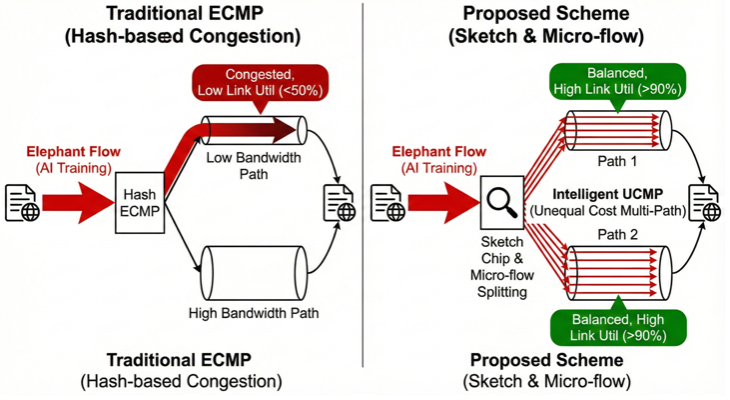
\includegraphics[width=30pc]{fig2.png}
\end{center}
\caption{\label{fig2}Comparison of Load Balancing Schemas: ECMP vs Micro-flow Awareness}
\end{figure}


Multiple equal-cost or non-equal-cost paths in a WAN have significant delay differentials. Let the candidate path set be $\mathcal{P} = \{p_1, p_2, \dots, p_k\}$, with the measured RTT of each path denoted as $\text{RTT}(p_i)$. To ensure that two consecutive packets forwarded via different paths within the same TCP/RDMA connection do not arrive out-of-order and trigger Go-Back-N retransmissions, the algorithm must strictly adhere to the Flowlet splitting gap theoretical boundary [14]. The time interval $\Delta T$ between consecutive packets $\text{Pkt}_n$ and $\text{Pkt}_{n-1}$ of the same flow must be strictly greater than the maximum relative one-way delay difference among the candidate paths in the WAN:
\begin{equation}
\Delta T > \frac{1}{2} \left( \max_{i \in P} \mathrm{RTT}(p_i) - \min_{j \in P} \mathrm{RTT}(p_j) \right).
\end{equation}

The router's NP chip continuously monitors the arrival timestamps of packets. Once the boundary condition of Equation (3) is met, a safe new Flowlet splitting point is deemed to have occurred. Subsequently, combined with the underlying SRv6 G-SID list, the UCMP algorithm is utilized for fine-grained scheduling. The probability weight $W(p_m)$ for selecting candidate path $p_m$ to carry the Flowlet strictly follows the proportional distribution of the real-time available bandwidth $B_{res}$ across the entire network:
\begin{equation}
W(p_m) = \frac{B_{res}(p_m)}{\sum_{i=1}^{k} B_{res}(p_i)}
\end{equation}


By integrating network-side hardware processing with flowlet splitting boundaries, this mechanism distributes large flows across high-capacity paths. This effectively prevents host-side NIC buffer exhaustion induced by long WAN RTTs, providing an algorithmic foundation for scaling AI workloads from single datacenters to geo-distributed WANs.


\section{SRv6 Tenant-Level Backpressure Mechanism to Overcome Long RTTs}


Traditional data center RDMA networks heavily rely on PFC mechanisms to achieve lossless transmission [15]. However, when the physical distance extends from within the data center to hundreds of kilometers in a wide area network (WAN) environment, the long RTT imposes fundamentally different constraints on congestion control. Based on flow control stability theory, this paper designs and implements a tenant-level in-band signaling backpressure architecture using SRv6, effectively resolving deadlocks and queue congestion issues in WANs.


\subsection{Backpressure Stability and BDP ``Blind Mode'' Modeling Under Long WAN Latencies}


In high-speed WANs, the long RTT significantly increases the BDP. We define the interval from when congestion occurs and backpressure signaling is initiated to when the upstream source receives the signal and stops transmission as the reaction time. Let the link capacity be $C$. During Blind Mode, a substantial volume of in-flight packets continues to flow into the node. The theoretical lower bound of this volume $V_{blind}$ is given by:
\begin{equation}
V_{blind} = C \times RTT
\end{equation}

% 修改
To quantitatively demonstrate the buffer implications under long WAN latencies, Table 1 summarizes the required blind-zone buffering across varying transmission distances and contrasts the operational behavior of standard PFC with our proposed End.X.PFC signaling.

\begin{table}[h]
\caption{\label{tab3}BDP Blind-zone buffer requirements and backpressure overhead across varying WAN distances.}
\begin{center}
\lineup
\small
\begin{tabular}{@{}>{\raggedright\arraybackslash}p{2.0cm}
                >{\centering\arraybackslash}p{1.2cm}
                >{\centering\arraybackslash}p{1.3cm}
                >{\raggedright\arraybackslash}p{1.7cm}
                >{\raggedright\arraybackslash}p{3.7cm}
                >{\raggedright\arraybackslash}p{3.9cm}@{}}
\br
\centering WAN Link Distance (km) & RTT ($\mu$s) & Link Bandwidth & \centering Theoretical $V_{blind}$ (BDP) & \centering Traditional PFC Behavior & \centering Proposed SRv6 End.X.PFC ($Q_{threshold}$) \tabularnewline
\mr
0.1 (Intra-DC) & $\approx$10 & 100 Gbps & $\approx$125 KB & Port-level PAUSE, Head-of-Line (HoL) blocking risk & Flow-level exact backpressure ($<$128 KB) \\
50 (Metro-WAN) & $\approx$500 & 100 Gbps & $\approx$6.25 MB & Buffer overflow / Deadlock propagation & Provisioned queue buffer ($\approx$6.5 MB), isolated tenant queue \\
100 (Production) & $\approx$1000 (1 ms) & 100 Gbps & $\approx$12.5 MB & Severe HoL blocking, victim flows stalled & Precise in-band End.X.PFC SID, zero packet loss, isolated halt \\
500 (Cross-region) & $\approx$5000 (5 ms) & 100 Gbps & $\approx$62.5 MB & Frequent PFC storms \& fabric deadlock & Multi-hop End.X.PFC upstream regulation \\
\br
\end{tabular}
\end{center}
\end{table}

By coupling in-network hardware processing with flowlet-splitting boundaries, our mechanism balances large flows across high-capacity paths. This design averts host-side NIC buffer exhaustion under high WAN RTTs, establishing an algorithmic foundation for geo-distributed AI computing.


\subsection{In-band Signaling Architecture Based on SRv6 End.X.PFC}


To prevent deadlock propagation and maximize throughput, flow control must shift from coarse port-level to fine-grained tenant-level granularity. However, most commodity WAN devices lack native hardware support for hop-by-hop micro-flow backpressure. To bridge this gap, we implement a network-layer in-band signaling mechanism compliant with recent IETF drafts. Specifically, we define a new SRv6 Endpoint Behavior: the End.X.PFC SID [17]. By leveraging explicit routing, the traffic path is fully embedded in the IPv6 Segment Routing Header (SRH), enabling the following capabilities:


1) Signaling Structure: Within the 128-bit End.X.PFC SID, the Locator encodes routing topology, while the Function and Argument fields are repurposed to explicitly map specific slice or logical queue IDs.


2) Reverse Traceability: Upon congestion, a downstream node pinpoints the exact upstream interface and queue by parsing the preceding SID in the SRH, overcoming the unidirectional forwarding limitations of traditional IP networks.


\subsection{Fine-grained Tenant-Level Backpressure Algorithm and State Machine Implementation}


Building upon the signaling architecture, we implement a constant-time, bounded-state fine-grained backpressure algorithm within the switches. The state machine executes in four core stages:


1) Stream ID Management: At the WAN edge, incoming tenant traffic is assigned a globally unique Stream ID, mapping it to a specific hardware slice sub-interface and logical queue.


2) Congestion Detection: The downstream NPU monitors per-tenant queue occupancy ($Q_{len}$). An alarm triggers when $Q_{len}$ reaches a critical threshold ($Q_{threshold}$), which is explicitly provisioned to absorb the blind-mode in-flight traffic ($V_{blind}$) dictated by the WAN BDP.


3) Precision Flow Control Message (PFCM) Generation: Rather than flooding the link with standard IEEE 802.1Qbb PAUSE frames, the congested node generates a Precision PFCM. This PFCM is encapsulated via an IPv6 Hop-by-Hop (HBH) or Destination Options Header (DOH) [18], addressed to the responsible upstream node's End.X.PFC SID.


4) Upstream Enforcement: Upon intercepting the End.X.PFC signal, the upstream device halts only the specific tenant's logical queue identified by the SID.


By elevating flow control from the Layer 2 MAC domain to the Layer 3 SRv6 logical slice domain, End.X.PFC isolates AI workloads without disrupting co-located tenant services. This design inherently eliminates the victim-flow phenomenon, ensuring lossless transmission and low tail latency even under severe Incast conditions.


\section{Service Awareness and Slice Hard Isolation Based on APN and SRv6 Data-Network Synergy}


To meet the stringent requirements of data element circulation and ensure strict compliance, the mechanism deeply integrates AAN technology with the underlying slicing architecture, thereby enhancing the network's awareness and responsiveness.


\subsection{Business Semantic Awareness and Deep APN Encapsulation}


When business data flows enter the intelligent WAN edge, devices perform deep inspection of flow characteristics to accurately identify their business attributes (e.g., sensitive medical records, large model training data). These high-dimensional semantics are then mapped to a standardized identifier---the APN ID. In accordance with standard encapsulation specifications, this APN ID is seamlessly embedded into the IPv6 packet's Hop-by-Hop Options Header or Destination Options Header, enabling the underlying network to recognize and interpret the specific business context of the packets it carries in real time.


\begin{figure}[h]
\begin{center}
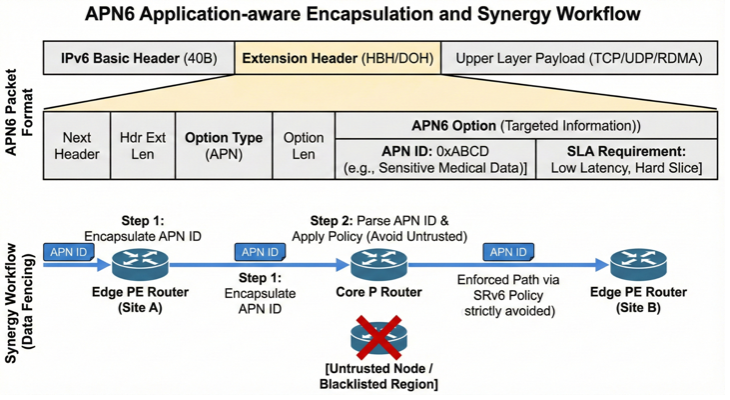
\includegraphics[width=30pc]{fig3.png}
\end{center}
\caption{\label{fig3}APN6 Application-aware Encapsulation and Synergy Workflow}
\end{figure}


\subsection{Slice Sub-interface Hard Isolation Guarantee}


Traditional networks predominantly rely on soft isolation techniques, wherein best-effort traffic can inadvertently exhaust shared buffer resources during severe congestion, thereby compromising high-priority transmissions. To satisfy the stringent zero-packet-loss requirements inherent to large-scale AI training, this approach integrates physical-layer slice sub-interface technology within the Enhanced VPN (VPN+) framework to achieve strict hardware-level isolation [19]. Through underlying hardware mechanisms, a single high-speed physical link is partitioned into mutually independent logical sub-interfaces. Each slice is deterministically bound to dedicated hardware queue resources and guaranteed physical bandwidth within the NPU. Consequently, even under conditions where background traffic experiences extreme congestion and packet loss, the dedicated slices accommodating critical AI workloads are able to sustain deterministic ultra-low latency and absolute zero packet loss.


\subsection{Compliant Routing and Data Fencing Based on APN}


In privacy protection scenarios, the APN ID functions as an identifier for data traversing the network. The control platform establishes strict security boundaries in advance. When sensitive data enters the network, the system triggers the Constrained Shortest Path First (CSPF) algorithm based on the security SLA requirements associated with the APN ID. This algorithm specifically computes a customized SRv6 explicit path that completely avoids any untrusted regions. As a result, sensitive data achieves isolation from non-compliant areas at the physical layer, effectively creating an invisible logical tunnel across the WAN.


\section{Production Network Deployment and Multi-Dimensional Performance Evaluation}


To rigorously quantify the real-world performance of this mechanism under underlying algorithm optimization and data-network synergy, we conducted large-scale testing and validation directly on the live intelligent wide-area production network built by us. The one-way physical distance of the test topology exceeded 100 kilometers, and the workloads comprehensively covered distributed training tasks of industry-mainstream LLM models.


\subsection{JCT and Model Training Computing Efficiency Evaluation}


In distributed AI training, the primary key performance indicator (KPI) of network efficiency is not bandwidth utilization alone, but rather JCT. As model parameter scales continue to grow, network congestion caused by Ring All-Reduce gradient synchronization exerts an increasingly significant impact on JCT, thereby substantially degrading end-to-end training performance.


To objectively evaluate system carrying capacity under varying network conditions, this experiment selects three representative models with different parameter scales: LLaMA-7B, LLaMA-13B, and GPT-175B, the latter imposing extremely high collective communication overhead due to its massive parameter volume.


The evaluation framework defines three controlled experimental groups:


1) Local-DC: A same-rack, short-reach environment with RTT $<$ 10$\mu$s and lossless transmission, representing an idealized intra-datacenter setting and serving as the upper-bound reference for achievable JCT.


2) Legacy WAN: A conventional wide-area network configuration employing host-side 5-tuple ECMP hash-based load balancing combined with standard port-level PFC.


3) Proposed Mechanism: A 100-km long-distance deployment that enables hardware-level Sketch-based micro-flow scheduling adapted to the LSQ architecture, together with a tenant-level backpressure control mechanism.


\begin{table}[h]
\caption{\label{tab1}Throughput and computing efficiency comparison of different scale large models (LLaMa/GPT) over a 100-km WAN.}
\begin{center}
\lineup
\small
\begin{tabular}{@{}>{\raggedright\arraybackslash}p{2.0cm}
                >{\raggedright\arraybackslash}p{3.2cm}
                >{\raggedleft\arraybackslash}p{2.2cm}
                >{\raggedleft\arraybackslash}p{3.5cm}@{}}
\br
\centering Model & \centering Configuration & \centering Throughput & \centering Efficiency Loss \tabularnewline
\centering (Params) & & \centering (Samples/s) & \centering (vs. Local-DC) \tabularnewline
\mr
LLaMa-7B & Local-DC (LAN Baseline) & 715.4 & 0.00\% \\
LLaMa-7B & Legacy WAN & 486.2 & $-$32.03\% \\
LLaMa-7B & Proposed Mechanism & 708.5 & $-$0.96\% \\
\mr
LLaMa-13B & Local-DC (LAN Baseline) & 412.8 & 0.00\% \\
LLaMa-13B & Legacy WAN & 265.1 & $-$35.78\% \\
LLaMa-13B & Proposed Mechanism & 406.3 & $-$1.57\% \\
\mr
GPT-175B & Local-DC (LAN Baseline) & 25.1 & 0.00\% \\
GPT-175B & Legacy WAN & 6.5 & $-$74.10\% (JCT collapses) \\
GPT-175B & Proposed Mechanism & 24.6 & $-$1.99\% \\
\br
\end{tabular}
\end{center}
\end{table}


The detailed experimental results in Table 1 indicate the following observations. For billion-parameter-scale models such as LLaMA-7B and LLaMA-13B, the Legacy WAN exhibits severe performance degradation due to hash-induced traffic polarization and delayed PFC congestion control. These factors lead to substantial GPU underutilization, with computational efficiency losses exceeding 30\%.


For ultra-large-scale models such as GPT-175B, the problem is further amplified by pronounced Incast traffic patterns during gradient synchronization. Under such conditions, the Legacy WAN exhibits severe system-level performance degradation, with throughput dropping by more than 74\%, which in turn leads to a multi-fold increase in JCT.


In contrast, when the proposed hardware scheduling and tenant-level backpressure mechanisms are fully enabled, the achieved throughput (samples/s) for both medium-scale and large-scale models closely approximates the ideal performance curve observed in Local-DC environments. Across a 100-km wide-area deployment, the overall computational efficiency loss is constrained to approximately 1.8\%.


These results strongly demonstrate that the proposed network-side hardware--algorithm co-design effectively mitigates communication bottlenecks induced by model scaling, thereby significantly reducing JCT under wide-area training scenarios.


\subsection{Tail Latency and Microscopic Queue Depth Analysis}


In distributed training systems, the AI network performance is not governed by average latency but is instead dominated by the ``slowest packet'' phenomenon. During synchronous iterations, tens of thousands of GPUs may be forced to idle while waiting for a single straggling packet delayed by network congestion, thereby significantly degrading cluster-level execution efficiency. Consequently, minimizing tail latency, particularly the 99th percentile (P99), is critical for maintaining training performance.


In this experiment, we further analyze the microscopic queue occupancy and tail latency behavior of the WAN core aggregation switch during the gradient synchronization phase of backpropagation.


\begin{table}[h]
\caption{\label{tab2}Evaluation of link utilization, maximum queue depth, and P99 tail latency under polarized elephant flow impacts.}
\begin{center}
\lineup
\small
\begin{tabular}{@{}>{\raggedright\arraybackslash}p{3.0cm}
                >{\raggedright\arraybackslash}p{3.2cm}
                >{\raggedright\arraybackslash}p{3.0cm}
                >{\raggedright\arraybackslash}p{2.8cm}@{}}
\br
\centering Load Balancing & \centering Avg. Link & \centering Max Queue Depth & \centering P99 Tail \tabularnewline
\centering Mechanism & \centering Utilization & \centering (M packets) & \centering Latency \tabularnewline
\mr
Legacy (Hash ECMP) & 45.8\% (Severe Resource Waste) & 4.8 M (Prolonged Near Overflow) & Surges over 300\%+ above baseline \\
\mr
Proposed (HW Sketch + UCMP) & 90.2\% (Extremely High Efficiency) & Reduced by $\sim$68\% & Approaches Ultra-Low Jitter LAN State \\
\br
\end{tabular}
\end{center}
\end{table}


As shown in Table 2, conventional ECMP routing under heavy elephant-flow workloads causes rapid queue buildup on core links, reaching peak depths of approximately 4.8M packets. This congestion frequently triggers upstream PAUSE frames, creating a feedback loop that severely inflates P99 tail latency.


In contrast, by leveraging the in-network LSQ-Sketch matrix for millisecond-level dynamic flow slicing, our mechanism elevates link utilization beyond 90\% while reducing peak queue depth by $\sim$68\% (to under 1.5M packets). This suppression of queue occupancy and P99 latency minimizes the network-layer ``straggler'' effect, bridging the compute-communication gap for distributed training.


Finally, isolation stress tests validate the efficacy of AAN slice-based sub-interfaces. Even when injected background traffic exceeds line rate and causes massive packet drops on the best-effort slice, the hardware-isolated AI slice maintains deterministic forwarding. It achieves zero packet loss and strict interference isolation, delivering a secure transport substrate for data-localized computing networks.


\section{Conclusion and future work}


As distributed LLM training scales across wide-area networks, traditional best-effort IP architectures suffer from flow-control instability, hash polarization, and inadequate application awareness. To address these bottlenecks, we propose a cross-plane lossless transmission architecture based on SRv6. At the data plane, we co-design in-network hardware with traffic scheduling, integrating an LSQ-assisted Sketch mechanism to resolve SRAM read-write contention under bursty ON/OFF traffic. By adhering to a rigorous temporal bound for flowlet segmentation, our UCMP scheduling circumvents the out-of-order Go-Back-N retransmission penalties typical of high-RTT WANs.


To guarantee lossless transmission, we introduce a tenant-level elastic backpressure mechanism via SRv6 End.X.PFC in-band signaling, inherently preventing global deadlocks. Concurrently, integrating AAN enforces hardware-level data isolation for strict regulatory compliance. Evaluations on a 100-km production WAN demonstrate that our system elevates link utilization from 45\% to over 90\%. By mitigating tail-latency inflation, the architecture restricts the computational efficiency loss of training massive models, such as GPT-175B, to approximately 1.8\%.


Future iterations will explore integrating Deep Reinforcement Learning (DRL) for autonomous forwarding-plane optimization, advancing toward fully self-adaptive routing networks [20].


\ack

The authors would like to thank the Century College, Beijing University of Posts and Telecommunications for providing the necessary research facilities and technical support for this study.


\section*{References}
\begin{thebibliography}{99}
\bibitem{ref1} Narayanan D, Shoeybi M, Casper J, et al. 2021 Efficient large-scale language model training on GPU clusters using megatron-LM \textit{Proc. Int. Conf. for High Performance Computing, Networking, Storage and Analysis (SC)} (St. Louis, MO, USA) pp 1--15
\bibitem{ref2} Hsieh K, Harlap A, Vijaykumar N, et al. 2017 Gaia: Geo-distributed machine learning approaching LAN speeds \textit{Proc. 14th USENIX Symp. on Networked Systems Design and Implementation (NSDI)} (Boston, MA, USA) pp 629--647
\bibitem{ref3} Guo C, Wu H, Tan K, et al. 2016 RDMA over commodity ethernet at scale \textit{Proc. ACM SIGCOMM 2016 Conf.} (Florianopolis, Brazil) pp 202--215
\bibitem{ref4} Mittal R, Lam V T, Dukkipati N, et al. 2015 TIMELY: RTT-based congestion control for the datacenter \textit{Proc. ACM SIGCOMM 2015 Conf.} (London, UK) pp 537--550
\bibitem{ref5} Liu Z, Bai W, Zhu H, et al. 2020 Congestion control for high-speed WANs \textit{IEEE/ACM Trans. Netw.} \textbf{28} 2154--2167
\bibitem{ref6} Al-Fares M, Loukissas A, Vahdat A. 2008 A scalable, commodity data center network architecture \textit{ACM SIGCOMM Comput. Commun. Rev.} \textbf{38} 63--74
\bibitem{ref7} Sapio A, Abdelmoniem A M, Anderson D, et al. 2021 Scaling distributed machine learning with in-network aggregation \textit{Proc. 18th USENIX Symp. on Networked Systems Design and Implementation (NSDI)} pp 785--808
\bibitem{ref8} Zhang H, Chen M, Bai W, et al. 2019 HPCC: high precision congestion control \textit{Proc. ACM SIGCOMM 2019 Conf.} (Beijing, China) pp 137--151
\bibitem{ref9} Cormode G and Muthukrishnan S. 2005 An improved data stream summary: the count-min sketch and its applications \textit{J. Algorithms} \textbf{55} 58--75
\bibitem{ref10} Chole S, Fingerhut A, Ma S, et al. 2017 DRMT: disaggregated programmable switching \textit{Proc. ACM SIGCOMM 2017 Conf.} (Los Angeles, CA, USA) pp 1--14
\bibitem{ref11} Dong P, Zheng W, Fang J, et al. 2020 SPArch: efficient architecture for sparse matrix multiplication \textit{Proc. 47th Annual Int. Symp. on Computer Architecture (ISCA)} (Valencia, Spain) pp 138--151
\bibitem{ref12} Sergeev A and Del Balso M. 2018 Horovod: fast and easy distributed deep learning in TensorFlow \textit{arXiv preprint} arXiv:1802.05799
\bibitem{ref13} Moshref M, Yu M, Govindan R, et al. 2014 DREAM: dynamic resource allocation for software-defined measurement \textit{Proc. ACM SIGCOMM 2014 Conf.} (Chicago, IL, USA) pp 419--430
\bibitem{ref14} Kandula S, Katabi D, Sinha S, et al. 2007 Dynamic load balancing without packet reordering \textit{ACM SIGCOMM Comput. Commun. Rev.} \textbf{37} 51--62
\bibitem{ref15} Stephens B, Cox A L, Singla A, et al. 2014 Practical DCB for improved data center networks \textit{Proc. IEEE INFOCOM 2014 Conf.} (Toronto, Canada) pp 1824--1832
\bibitem{ref16} Lu G, Miao R, Xiong Y, et al. 2022 RoCEv2 with concurrency control \textit{Proc. ACM SIGCOMM 2022 Conf.} (Amsterdam, Netherlands) pp 12--25
\bibitem{ref17} Filsfils C, Camarillo P, Leddy J, et al. 2021 IPv6 segment routing \textit{IETF RFC} 8986
\bibitem{ref18} Li Z, Peng S, Voyer D, et al. 2022 Application-aware Networking (APN) framework \textit{IETF Internet-Draft}
\bibitem{ref19} Foukas X, Patounas G, Elmokashfi A, et al. 2017 Network slicing in 5G: Survey and challenges \textit{IEEE Commun. Mag.} \textbf{55} 94--100
\bibitem{ref20} Valadarsky A, Schapira M, Shahaf D, et al. 2017 Learning to route \textit{Proc. 16th ACM Workshop on Hot Topics in Networks (HotNets)} (Palo Alto, CA, USA) pp 74--80
\end{thebibliography}
\end{document}